\label{3_algoritmo_genetico}

O pseudocódigo tradicional de um algoritmo evolutivo pode ser dado por \cite{algoritmopseudo}:

\begin{algorithm}[H]
$\textbf{AG(} fitness \textbf{)}$
\Begin{
	$P \gets InicializarPopulacao(fitness)$\;
	$P.fitness()$\;
	$t = 0$\;
	\While{t < número de gerações} {
		$Pais \gets Selecao(P)$\;
		$Filhos \gets Crossover(Pais)$\;
		$P \gets P \cup Filhos$\;
		$Mutacao(P)$\;
		$P.fitness()$\;
		$P \gets Sobrevivem(P)$\;
	}
}
\caption{Pseudocódigo do Algoritmo Genético.}
\label{alg:ag}
\end{algorithm}

Cada uma destas funções principais pode ser feita de diferentes maneiras. No entanto, tais implementações independem do problema a ser resolvido, o que torna sua confecção e manutenção bem mais simples.

\section{Seleção}

A escolha dos pais é feita por.

\section{Crossover}

Escolhidos os pais, optou-se neste trabalho por embaralhá-los aleatoriamente numa lista e, escolhendo-os dois a dois, verificar se os dois pais serão cruzados, de acordo com uma probabilidade $p_c$. Se sim, os pais terão seus materiais genéticos misturados por uma ação chamada \emph{crossover}.

Crossover envolve a quebra da sequência de genes de dois indivíduos em um mesma secção, com a subsequente troca de material na região delimitada por esta secção. Este trabalho se utilizou do crossover em dois pontos, o qual divide as sequências em duas partes distintas, ocorrendo troca do material genético entre estas partes. Tal ação é mostrada na figura \ref{fig:evolution-framework}.

\begin{figure}[ht!]
    \centering 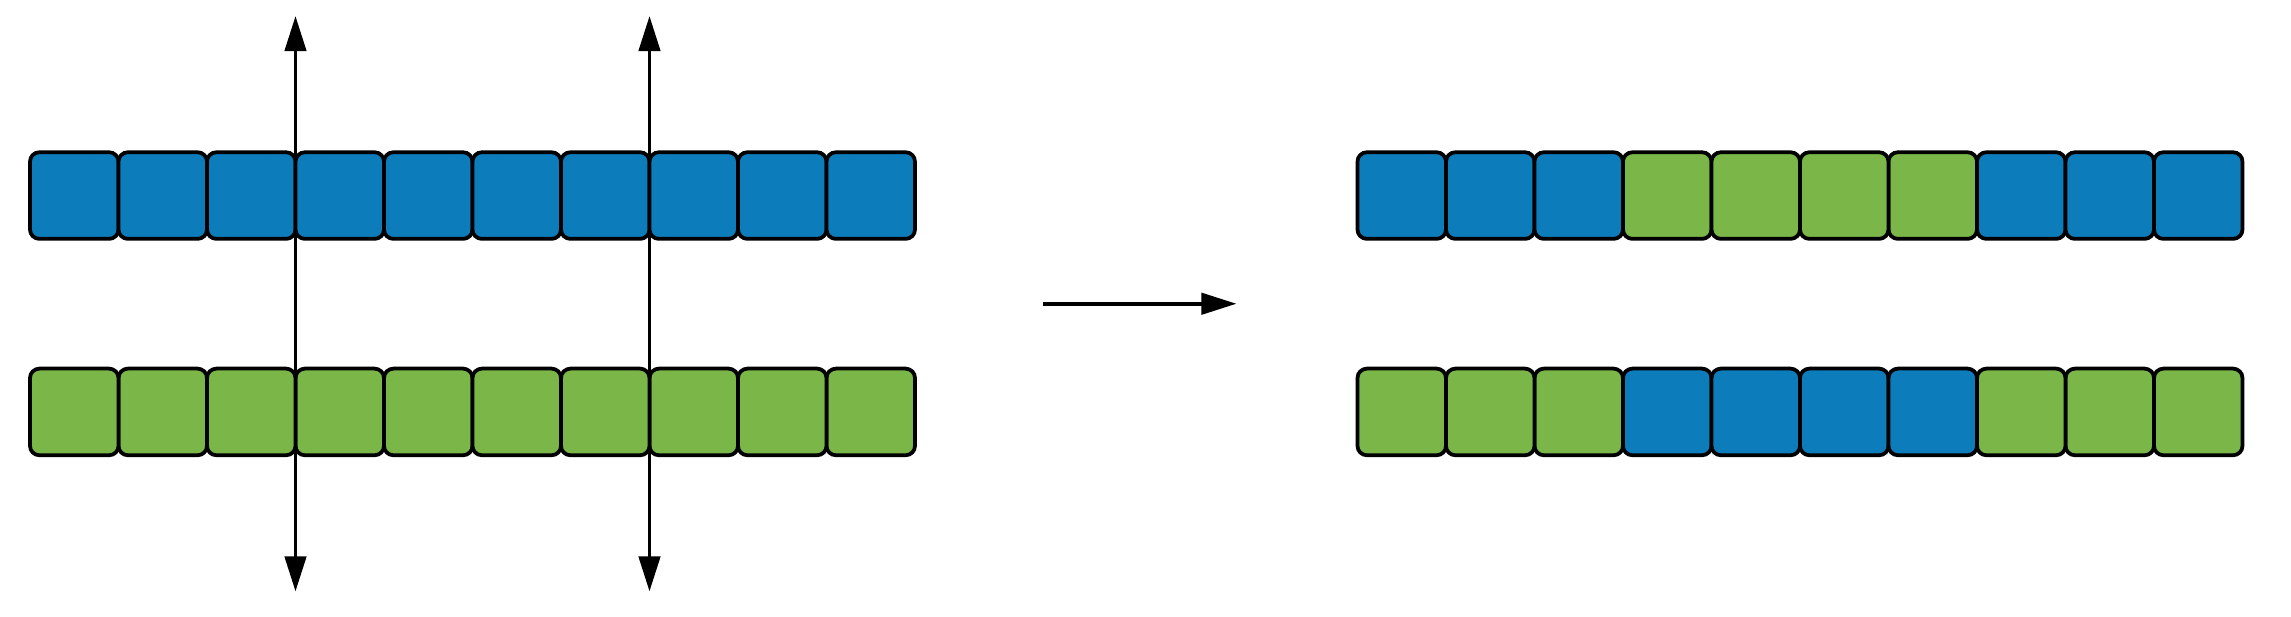
\includegraphics[width=1.0\textwidth]{crossover.png}
    \caption{Ação de crossover em dois pontos.}
    \label{fig:crossover}
\end{figure}

Toda ação de crossover gera duas sequências de genes (filhas) novas a partir das sequências originais (pais), adicionando dois indivíduos novos a cada crossover bem sucedido.

\section{Mutação}

A ação de mutação funciona, em sua estrutura mais básica, da seguinte forma: itera-se sobre todos os genes da população um a um. Com uma probabilidade $p_m$, é avaliado se o gene deveria ou não alterar sua expressividade. Se sim, o gene tem seu valor alterado aleatoriamente.

\section{Sobrevivência}

Texto.

